\documentclass[11pt]{article}
\usepackage[margin=2.2cm]{geometry}
\usepackage{booktabs}
\usepackage{amsmath,amssymb}
\usepackage[most]{tcolorbox}
\usepackage{xcolor}
\usepackage{graphicx}
\usepackage{enumitem}

\definecolor{wallred}{RGB}{180,0,0}

\newtcolorbox{diagnosis}{colback=red!5!white, colframe=red!40!black,
  fonttitle=\bfseries, boxrule=0.5pt, arc=2pt}
\newtcolorbox{tested}{colback=yellow!5!white, colframe=yellow!50!black,
  fonttitle=\bfseries, title=What We Tested, boxrule=0.5pt, arc=2pt}
\newtcolorbox{conclusion}{colback=blue!5!white, colframe=blue!50!black,
  fonttitle=\bfseries, title=Conclusion, boxrule=0.5pt, arc=2pt}

\title{\textbf{The Walls --- What We Know and Don't Know}\\[4pt]
\large Scaling Limitations of Neural Polar MAC Decoders}
\author{}
\date{April 2026}

\begin{document}
\maketitle
\thispagestyle{empty}

%% ============================================================
\section{Wall A: GMAC Class B at $N = 256$ (NCG Sequential Decoder)}

\begin{diagnosis}[title=Symptom]
NCG BLER \textbf{0.023} vs.\ SC BLER \textbf{0.006} --- a \textbf{4.5$\times$} gap at $N = 256$.
At $N = 512$: NCG 0.012 vs.\ SC ${\sim}$0.001 (12$\times$).
At $N = 1024$: NCG 0.47 (essentially broken).
The decoder works fine at $N \le 128$ (NCG/SC $\approx 1.0$).
\end{diagnosis}

\begin{tested}
\begin{enumerate}[nosep,leftmargin=*]
  \item \textbf{Exposure bias:} Compared teacher-forced vs.\ free-running mutual information at $N = 32$. They match --- exposure bias is not the cause at small $N$, but may compound at large $N$.
  \item \textbf{Cascade amplification:} Checked BER/BLER ratio for NCG vs.\ SC. They are similar --- errors are not cascading differently.
  \item \textbf{First-error localization:} Top-5 first-error positions are NCG-specific (the model has specific weak spots), but the remaining errors are broadly distributed across positions.
  \item \textbf{Lower rate:} Tested multiple rates. The gap persists at all rates tested.
  \item \textbf{Scheduled sampling:} Trained with mixed teacher-forced / free-running schedule. Only 21\% BLER improvement (0.023 $\to$ 0.018), still far from SC.
  \item \textbf{Learning rate continuation:} lr $= 10^{-3}$ destroyed the model; lr $= 10^{-4}$ showed no improvement.
\end{enumerate}
\end{tested}

\begin{conclusion}
Likely a \textbf{fundamental limitation of sequential NCG} at this scale.
The model converges to a local minimum it cannot escape.
The $d = 16$ embedding dimension may be insufficient to represent the $2^{256}$-sized codebook structure, but increasing $d$ did not help either (training becomes harder).

\medskip
\textbf{What we don't know:} Whether a fundamentally different training strategy (e.g., reinforcement learning, or a non-autoregressive architecture) could break through this wall.

\medskip
\textbf{Note:} CRC-SCL $L = 4$ has no such wall (BLER $< 10^{-4}$ at $N = 256$), suggesting the issue is specific to the sequential neural approach, not to the channel/code combination.
\end{conclusion}

\begin{figure}[h]\centering
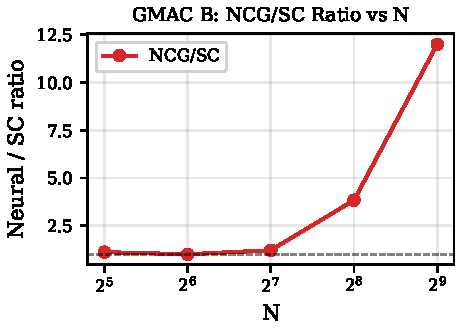
\includegraphics[width=0.75\textwidth]{plot_wall_gmac.pdf}
\end{figure}

%% ============================================================
\section{Wall B: ISI-MAC at $N = 512$ (NPD Chained Decoder)}

\begin{diagnosis}[title=Symptom]
Best NPD BLER at $N = 512$: not evaluated (all architectures failed at $N = 256+$).\\
At $N = 128$: NPD 0.030 vs.\ chained trellis SC 0.022 (1.35$\times$ gap, already losing).\\
At $N = 256$: NPD 0.011 vs.\ chained SC 0.006 (1.84$\times$).\\
Contrast: NPD \textbf{beats} chained SC at $N \le 64$ by 19--32\%.
\end{diagnosis}

\begin{tested}
\begin{enumerate}[nosep,leftmargin=*]
  \item \textbf{Architecture sweep:} 8 configurations tested (GRU/LSTM, $h \in \{128, 256, 512\}$, per-depth MLPs, pointwise MLPs). None helped at $N \ge 128$.
  \item \textbf{Memorization test:} The model \emph{can} represent $N = 512$ (passes memorization on small batches). The issue is generalization, not capacity.
  \item \textbf{First-error analysis:} 84\% of NPD errors occur in the last quarter (positions 385--512). The BiGRU loses track of state over long sequences.
  \item \textbf{Rate sweep:} Tested multiple rates. The gap persists.
  \item \textbf{Embedding dimension:} d=16 h=100 vs.\ d=64 h=128 --- similar loss at $N = 512$. Hidden width $h$ matters more than embedding dimension $d$.
  \item \textbf{Comparison to paper:} Aharoni et al.\ use d=8 \emph{pointwise} MLP for single-user and achieve good results at $N = 1024$. We need BiGRU for MAC because the two-user interaction requires richer representations.
  \item \textbf{3-phase design at $N = 64$:} Works but did not outperform the GMAC-proxy frozen set.
\end{enumerate}
\end{tested}

\begin{conclusion}
$N = 512$ MAC is \textbf{fundamentally harder than $N = 1024$ single-user}.
The chained approach (Stage 1 marginalizes $V$ as noise) creates a harder effective channel for $U$-decoding --- the neural decoder must implicitly learn a more complex posterior.
The BiGRU's hidden state degrades over 512 sequential positions.

\medskip
\textbf{What we don't know:}
\begin{itemize}[nosep]
  \item Whether a Transformer-based architecture (with attention over all positions) could maintain long-range dependencies better.
  \item Whether joint (non-chained) neural decoding --- decoding $U$ and $V$ simultaneously --- would avoid the noise-marginalization bottleneck.
  \item Whether stronger ISI ($h > 0.3$) makes the problem easier or harder for NPD.
\end{itemize}
\end{conclusion}

\begin{figure}[h]\centering
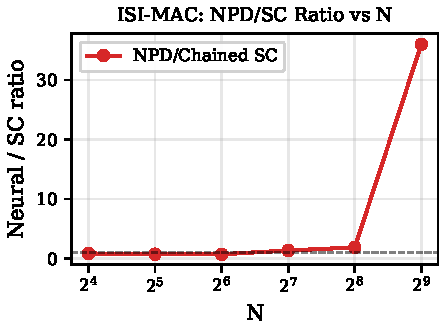
\includegraphics[width=0.75\textwidth]{plot_wall_isi.pdf}
\end{figure}

%% ============================================================
\section{Common Pattern Across All Walls}

\begin{center}\small
\begin{tabular}{@{}l c c c l@{}}
\toprule
Channel & Wall $N$ & NPD/SC at wall & Architecture & Root cause hypothesis \\
\midrule
GMAC B   & 256 & 4.5$\times$  & NCG d=16   & Sequential local minimum \\
ISI-MAC  & 128+ & 1.35$\times$ & NPD BiGRU  & State degradation over length \\
MA-AGN   & 32  & 1.6$\times$  & NPD BiGRU  & Weak memory + chained marginalization \\
Ising    & 16  & 1.04$\times$ & NPD BiGRU  & Channel too lossy \\
\bottomrule
\end{tabular}
\end{center}

\noindent Five observations that hold across all walls:
\begin{enumerate}[nosep]
  \item \textbf{Works at small $N$, gap grows with $N$.} The neural decoder handles short codes well but struggles to scale.
  \item \textbf{Not a capacity issue.} Memorization tests pass --- the model can represent the solution.
  \item \textbf{Not purely architectural.} Many configurations tested (GRU, LSTM, MLP, per-depth, varying $d$ and $h$).
  \item \textbf{More training helps but plateaus.} Loss curves flatten; longer training does not close the gap.
  \item \textbf{Hidden width $h$ matters more than embedding dim $d$.} Going from $h = 64$ to $h = 100$ helps; $d = 16$ to $d = 64$ does not.
\end{enumerate}

\medskip
\noindent\textbf{Honest assessment:} We do not have a clear path to breaking these walls with the current architecture. The most promising directions are:
\begin{itemize}[nosep]
  \item Non-autoregressive or partially parallel decoding
  \item Attention-based architectures for long-range dependencies
  \item Hybrid decoders (neural for hard positions, analytical for easy ones)
  \item Joint two-user neural decoding (avoid chained marginalization)
\end{itemize}

\end{document}
